\documentclass[11pt]{article}

% ---------------------------------------------------------------------------
% Packages
% ---------------------------------------------------------------------------
\usepackage[margin=1in]{geometry}
\usepackage{amsmath,amssymb,amsthm}
\usepackage{graphicx}
\usepackage{booktabs}
\usepackage{multirow}
\usepackage{array}
\usepackage{siunitx}
\usepackage{caption}
\usepackage{subcaption}
\usepackage[table]{xcolor}
\usepackage{enumitem}
\usepackage{titlesec}
\usepackage{float}
\usepackage{tikz}
\usepackage{pgfplots}
\pgfplotsset{compat=1.18}
\usetikzlibrary{arrows.meta,positioning,fit,backgrounds,calc,shapes.geometric,
                shadows.blur,decorations.pathreplacing,patterns}
\usepackage[font=small,labelfont=bf,width=0.92\textwidth]{caption}
\usepackage{hyperref}
\hypersetup{colorlinks=true,linkcolor=blue!45!black,citecolor=blue!45!black,
            urlcolor=blue!45!black}

\titleformat{\section}{\large\bfseries}{\thesection}{0.6em}{}
\titleformat{\subsection}{\normalsize\bfseries}{\thesubsection}{0.6em}{}
\graphicspath{{figures/}}
\captionsetup[subfigure]{labelfont=normalfont}

% siunitx column for numeric alignment
\sisetup{detect-weight=true,detect-family=true}
\newcolumntype{N}{S[table-format=3.2]}

% Palette (Okabe--Ito, matches the matplotlib figures)
\definecolor{cblue}{HTML}{0072B2}
\definecolor{corange}{HTML}{E69F00}
\definecolor{cgreen}{HTML}{009E73}
\definecolor{cred}{HTML}{D55E00}
\definecolor{cpurple}{HTML}{CC79A7}
\definecolor{cgray}{HTML}{6E6E6E}
\definecolor{cbg}{HTML}{F4F6F8}

\newcommand{\E}{\mathbb{E}}
\newcommand{\best}[1]{\textbf{#1}}

% ---------------------------------------------------------------------------
\title{\textbf{Mitigating Catastrophic Forgetting in CT-Based\\
Abdominal-Trauma Detection:\\[2pt]
\large A Comparison of EWC, Experience Replay, and Their Combination}}
\author{}
\date{Technical Report - \today}

\begin{document}
\maketitle
\vspace{-2.2em}
\begin{center}\rule{0.6\textwidth}{0.4pt}\end{center}

\begin{abstract}
\noindent
We examine catastrophic forgetting in a convolutional classifier trained on a
sequence of tasks drawn from the RSNA~2023 Abdominal Trauma Detection dataset,
and compare three common mitigation strategies against plain fine-tuning:
Elastic Weight Consolidation (EWC), Experience Replay, and a combination of the
two. We report two settings. Under class-incremental training, we observe that
fine-tuning and EWC both forget almost completely ($100\%$), that Replay brings
forgetting down to $86.75\%$, and that the combined method attains the lowest
forgetting we measured ($\best{29.50\%}$) while largely giving up its ability to
learn the new task. We read this as an illustration of the stability--plasticity
trade-off rather than as a ranking of methods. Under window-based
domain-incremental training, Replay gives the best average accuracy
($\best{57.71\%}$), yet every method stays close to chance, which suggests that
the binding constraint in that setting is representation learning rather than
forgetting. We state each method and metric formally, report the results with
figures and tables, and describe a set of changes that this reading leads us to
implement for the next round of experiments.
\end{abstract}

% ===========================================================================
\section{Introduction}
% ===========================================================================
\subsection{Motivation}
Contrast-enhanced computed tomography (CT) is a standard tool for assessing
abdominal trauma, and there is steady interest in models that can flag likely
injury on a CT study. A useful model, however, is not finished at the moment it
is trained. Scanners are replaced, acquisition protocols are revised, and the
clinical question itself tends to grow more specific over time, for instance from
whether any injury is present to which organ is involved and how severe it is. A
deployed model is therefore expected to keep learning after release.

This is harder than it first appears, mainly because the original training data
is usually not available later. Image archives are pruned for storage, and
patient-privacy rules limit how long identifiable images may be kept and how
freely they may move between sites~\cite{lee2020clcardiac}. The model often has to
be updated from whatever new data is on hand, with little or no access to the
historical set. Retraining from scratch on all data combined would be the simple
fallback, but it is the option these constraints tend to remove.

Updating a network on new data alone runs into a familiar difficulty. When a
network is trained on one task and then on another, the updates for the second
task move the weights wherever the new loss decreases, with nothing to preserve
the function learned for the first, and accuracy on the earlier task can fall
sharply. McCloskey and Cohen called this \emph{catastrophic
forgetting}~\cite{mccloskey1989}, and French attributed it to the same property
that lets these networks generalise, namely that their representations are
distributed, so the weights that hold old knowledge are also the ones a new task
adjusts~\cite{french1999}. \emph{Continual learning} (also called lifelong or
incremental learning) is the body of work concerned with updating a model over a
stream of tasks while retaining what it has already learned~\cite{delange2021survey}.

\subsection{Scope and contributions}
We ask a concrete version of this question: do the two most widely used remedies,
Elastic Weight Consolidation (EWC) and Experience Replay, actually prevent
forgetting when a CNN learns to detect abdominal trauma on CT slices one task at
a time? We study four methods, plain fine-tuning, EWC, Replay, and the
combination EWC+Replay, under two ways of constructing the task stream. Our
contributions are:
\begin{enumerate}[leftmargin=1.7em,topsep=2pt,itemsep=2pt]
  \item a self-contained, reproducible comparison of the four methods on the
        RSNA~2023 Abdominal Trauma dataset, with every metric defined formally
        (Sections~\ref{sec:methods}--\ref{sec:metrics});
  \item evidence that, in the class-incremental setting, only methods that revisit
        old data (Replay, and EWC+Replay) reduce forgetting, while a pure
        weight-space penalty (EWC) does not (Section~\ref{sec:results});
  \item a diagnosis of why a second, window-based task stays at chance, isolating
        representation quality rather than forgetting as the limiting factor
        (Section~\ref{sec:analysis}); and
  \item a set of six concrete, implemented changes that follow from this
        diagnosis (Section~\ref{sec:mods}).
\end{enumerate}

\subsection{Background and key terms}
Before the formal treatment we fix the vocabulary used throughout.
\begin{description}[leftmargin=0pt,labelindent=0pt,style=nextline,topsep=2pt,itemsep=3pt]
  \item[Task and the task stream.] A \emph{task} is one stage of training with its
        own data and (possibly) its own classes. The model meets the tasks in
        order, $\mathcal{T}_1,\mathcal{T}_2,\dots$, and we never reset it between
        them.
  \item[Three continual-learning scenarios.] The literature distinguishes
        \emph{task-incremental} learning (a task label is given at test time),
        \emph{domain-incremental} learning (the input distribution changes but the
        label set does not), and \emph{class-incremental} learning (new classes
        appear and no task label is given at test time). Class-incremental is the
        hardest of the three, because the model must tell apart classes it never
        saw together~\cite{delange2021survey}. We use a class-incremental setting
        (Experiment~1) and a domain-incremental one (Experiment~2).
  \item[Catastrophic forgetting.] The drop in accuracy on an earlier task caused
        by training on a later one.
  \item[Stability and plasticity.] \emph{Stability} is the ability to retain old
        knowledge; \emph{plasticity} is the ability to acquire new knowledge. The
        two pull against each other, and balancing them is the central difficulty
        of continual learning, often called the \emph{stability--plasticity
        dilemma}.
  \item[Backward transfer.] The opposite of forgetting: when learning a later task
        \emph{improves} an earlier one. It shows up as a negative forgetting score.
\end{description}

% ===========================================================================
\section{Problem Setup and Notation}
% ===========================================================================
Let the model be a parametric classifier $f_\theta:\mathcal{X}\to
\mathbb{R}^{C}$ with parameters $\theta\in\mathbb{R}^d$ and $C$ classes.
Training runs over a sequence of $T$ tasks
$\mathcal{T}_1,\dots,\mathcal{T}_T$, where task $t$ supplies
$\mathcal{D}_t=\{(x_i^{(t)},y_i^{(t)})\}_{i=1}^{n_t}\sim\mathcal{P}_t$. While
training on task $t$, the learner sees all of $\mathcal{D}_t$ but none of
$\mathcal{D}_{1:t-1}$, save for whatever a small replay buffer happens to hold
(Fig.~\ref{fig:taskstream}). The per-task objective is the empirical
cross-entropy risk
\begin{equation}
\mathcal{L}_t(\theta)=
\frac{1}{n_t}\sum_{i=1}^{n_t}\ell\!\big(f_\theta(x_i^{(t)}),y_i^{(t)}\big),
\qquad
\ell(z,y)=-\log\frac{\exp(z_y)}{\sum_{c=1}^{C}\exp(z_c)} .
\label{eq:ce}
\end{equation}
Here $n_t$ is the number of training examples in task $t$; $(x_i^{(t)},y_i^{(t)})$
is the $i$-th image--label pair of that task; $f_\theta(x)\in\mathbb{R}^{C}$ is
the vector of class scores (logits) the model assigns to input $x$; in the loss
$\ell(z,y)$, $z=f_\theta(x)$ is that logit vector, $z_y$ its entry for the true
class $y$, and $z_c$ its entry for class $c$, so the fraction is the softmax
probability of the correct class and $\ell$ its negative log. A purely sequential
learner minimises only $\mathcal{L}_t$ at step $t$, and that single-task focus is
what drives forgetting.

\begin{figure}[H]
\centering
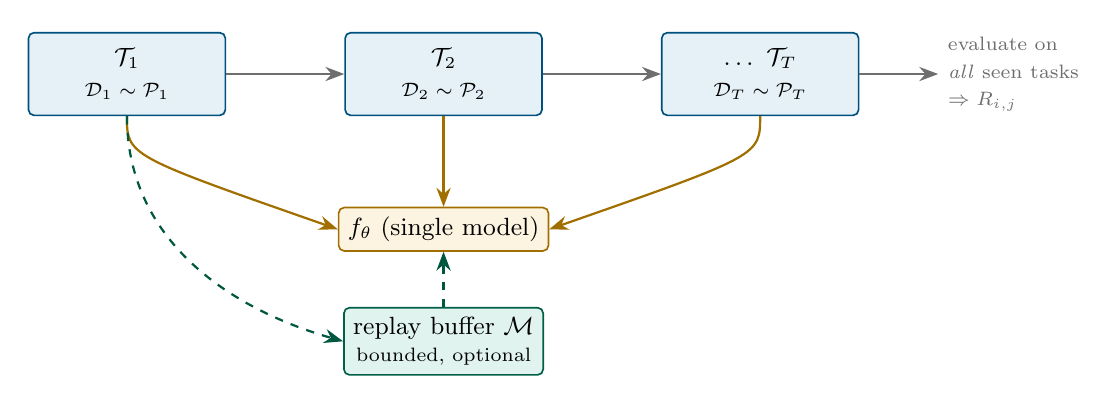
\begin{tikzpicture}[
  font=\small,
  task/.style={rounded corners=2pt,draw=cblue!70!black,fill=cblue!10,
               minimum width=2.5cm,minimum height=1.05cm,align=center,line width=0.6pt},
  mem/.style={rounded corners=2pt,draw=cgreen!60!black,fill=cgreen!12,
              minimum width=2.0cm,minimum height=0.7cm,align=center,line width=0.6pt},
  arr/.style={-{Stealth[length=2.4mm]},line width=0.8pt,cgray}]
  \node[task] (t1) {$\mathcal{T}_1$\\\scriptsize $\mathcal{D}_1\sim\mathcal{P}_1$};
  \node[task,right=1.5cm of t1] (t2) {$\mathcal{T}_2$\\\scriptsize $\mathcal{D}_2\sim\mathcal{P}_2$};
  \node[task,right=1.5cm of t2] (t3) {$\dots\ \mathcal{T}_T$\\\scriptsize $\mathcal{D}_T\sim\mathcal{P}_T$};
  \draw[arr] (t1) -- (t2);
  \draw[arr] (t2) -- (t3);
  % model passing through
  \node[draw=corange!70!black,fill=corange!12,rounded corners=2pt,
        below=1.15cm of t2,minimum width=2.4cm,line width=0.6pt] (model)
        {$f_\theta$ (single model)};
  \draw[arr,corange!70!black] (t1.south) .. controls +(0,-0.5) .. (model.west);
  \draw[arr,corange!70!black] (t2.south) -- (model.north);
  \draw[arr,corange!70!black] (t3.south) .. controls +(0,-0.5) .. (model.east);
  % replay buffer
  \node[mem,below=0.7cm of model] (buf) {replay buffer $\mathcal{M}$\\[-1pt]\scriptsize bounded, optional};
  \draw[arr,cgreen!55!black,dashed] (t1.south) .. controls +(0,-1.6) and +(-1.4,0.4) .. (buf.west);
  \draw[arr,cgreen!55!black,dashed] (buf.north) -- (model.south);
  % eval bracket
  \node[right=1.0cm of t3,align=left,text=cgray] (ev)
     {\scriptsize evaluate on\\[-1pt]\scriptsize \emph{all} seen tasks\\[-1pt]\scriptsize $\Rightarrow R_{i,j}$};
  \draw[arr] (t3) -- (ev);
\end{tikzpicture}
\caption{Continual-learning protocol. One model $f_\theta$ is trained on tasks
$\mathcal{T}_1,\dots,\mathcal{T}_T$ in sequence. Past data is unavailable apart
from an optional bounded replay buffer $\mathcal{M}$. After each task we test the
model on every task seen so far, which fills the accuracy matrix $R_{i,j}$.}
\label{fig:taskstream}
\end{figure}

\paragraph{Task constructions.}
\begin{itemize}[leftmargin=1.4em,topsep=2pt,itemsep=2pt]
  \item \textbf{Class-incremental (Experiment~1).} $T{=}2$. Task~1 shows only the
        no-injury class and Task~2 only the injury class. At test time there is
        no task identifier, so the model has to keep both decision regions intact
        at once.
  \item \textbf{Window-based domain-incremental (Experiment~2).} $T{=}3$. The
        same images and labels come back under three CT windows (Brain, Lung,
        Soft-tissue). Each task shifts the input distribution $\mathcal{P}_t$
        while leaving the label space unchanged.
\end{itemize}

% ===========================================================================
\section{Methods}\label{sec:methods}
% ===========================================================================
Figure~\ref{fig:methodflow} shows how the four methods tie consecutive tasks
together. The equations follow. Each method changes only how the loss for the
current task is formed; the optimiser, architecture, and data are otherwise
identical, so any difference in the results is attributable to the method.

\begin{figure}[H]
\centering
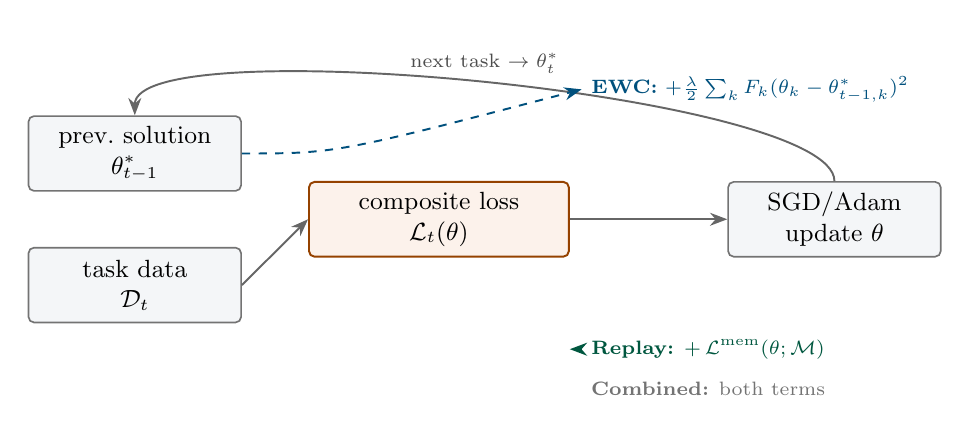
\begin{tikzpicture}[
  font=\small,
  box/.style={rounded corners=2pt,draw=black!55,fill=cbg,align=center,
              minimum height=0.95cm,minimum width=2.7cm,line width=0.6pt},
  loss/.style={rounded corners=2pt,draw=cred!70!black,fill=cred!8,align=center,
               minimum height=0.95cm,minimum width=3.3cm,line width=0.7pt},
  arr/.style={-{Stealth[length=2.2mm]},line width=0.7pt,black!60}]
  \node[box] (prev) {prev.\ solution\\$\theta^{*}_{t-1}$};
  \node[box,below=0.7cm of prev] (data) {task data\\$\mathcal{D}_t$};
  % central loss
  \node[loss,right=2.2cm of $(prev)!0.5!(data)$] (L) {composite loss\\$\mathcal{L}_t(\theta)$};
  \node[box,right=2.0cm of L] (upd) {SGD/Adam\\update $\theta$};
  \draw[arr] (data.east) -- (L.west);
  \draw[arr] (L.east) -- (upd.west);
  \draw[arr] (upd.north) .. controls +(0,1.1) and +(0,1.1) .. node[above,black!70,font=\scriptsize]{next task $\to\theta^{*}_{t}$} (prev.north);
  % method annotations on the loss
  \node[align=left,right=0.15cm of L,yshift=1.65cm,font=\scriptsize,text=cblue!70!black] (ewc)
    {\textbf{EWC:} $+\frac{\lambda}{2}\sum_k F_k(\theta_k-\theta^{*}_{t-1,k})^2$};
  \node[align=left,right=0.15cm of L,yshift=-1.65cm,font=\scriptsize,text=cgreen!55!black] (rep)
    {\textbf{Replay:} $+\,\mathcal{L}^{\mathrm{mem}}(\theta;\mathcal{M})$};
  \draw[arr,cblue!70!black,dashed] (prev.east) .. controls +(1.2,0) .. (ewc.west);
  \draw[arr,cgreen!55!black,dashed] (rep.west) -- (L.east|-rep.west);
  \node[font=\scriptsize,below=0.05cm of rep,text=black!55,align=left]
    {\textbf{Combined:} both terms};
\end{tikzpicture}
\caption{How each method changes the per-task objective. Baseline uses
$\mathcal{L}_t$ on its own. EWC adds a Fisher-weighted quadratic anchor to the
previous solution $\theta^{*}_{t-1}$. Replay adds a loss term over the memory
buffer $\mathcal{M}$. The combined method carries both terms.}
\label{fig:methodflow}
\end{figure}

\subsection{Baseline: sequential fine-tuning}
At task $t$ we update the parameters on $\mathcal{L}_t$ alone,
$\theta\leftarrow\arg\min_\theta\mathcal{L}_t(\theta)$. Nothing links one task to
the next, so this serves as the reference point against which we measure
forgetting.

\subsection{Elastic Weight Consolidation (EWC)}
EWC~\cite{kirkpatrick2017} takes the posterior after task $t{-}1$ as a Gaussian
prior for task $t$, with its precision set by the diagonal Fisher information,
\begin{equation}
F_k=\frac{1}{N}\sum_{i=1}^{N}
\left(\frac{\partial\log p_\theta(y_i\mid x_i)}{\partial\theta_k}\right)^{\!2}
\Bigg|_{\theta=\theta^{*}_{t-1}},
\label{eq:fisher}
\end{equation}
where $F_k$ is the (diagonal) Fisher information for parameter $k$, a measure of
how sharply the model's predictions depend on that weight; $N$ is the number of
samples $(x_i,y_i)$ drawn from task $t{-}1$ used to estimate it; $p_\theta(y\mid
x)$ is the model's predicted probability of label $y$ given input $x$; $\theta_k$
is the $k$-th model parameter; and $\theta^{*}_{t-1}$ are the parameters at which
task $t{-}1$ converged, i.e.\ the point at which the gradient is evaluated. The
objective then adds a quadratic penalty that pins down the weights the Fisher
term marks as important,
\begin{equation}
\mathcal{L}^{\text{EWC}}_t(\theta)=\mathcal{L}_t(\theta)
+\frac{\lambda}{2}\sum_k F_k\,(\theta_k-\theta^{*}_{t-1,k})^2 .
\label{eq:ewc}
\end{equation}
Here $\mathcal{L}_t(\theta)$ is the current-task loss of Eq.~\eqref{eq:ce}; the
sum over $k$ runs over all model parameters; $\lambda\ge 0$ is the regularisation
strength that sets how strongly the model is held near its previous solution; and
$F_k$ and $\theta^{*}_{t-1,k}$ are as defined for Eq.~\eqref{eq:fisher}.
A large $\lambda$ guards old knowledge at the expense of new learning. With more
than one past task the penalties simply add up, as
$\sum_{s<t}\frac{\lambda}{2}\sum_k F_k^{(s)}(\theta_k-\theta^{*}_{s,k})^2$. EWC
belongs to a wider family of prior-based methods; Synaptic
Intelligence~\cite{zenke2017si} replaces the Fisher term with an online estimate
of each weight's contribution to the loss, but keeps the same quadratic-anchor
form.

\subsection{Experience Replay}
Replay keeps a bounded buffer $\mathcal{M}=\bigcup_{s<t}\mathcal{M}_s$ of past
examples, $B$ per task, filled in reservoir fashion. During task $t$ the loss
mixes new and replayed data,
\begin{equation}
\mathcal{L}^{\text{rep}}_t(\theta)=
\underbrace{\frac{1}{|\mathcal{B}_t|}\!\!\sum_{(x,y)\in\mathcal{B}_t}\!\!
   \ell(f_\theta(x),y)}_{\text{current task}}
+\underbrace{\frac{1}{|\mathcal{B}_\mathcal{M}|}\!\!
   \sum_{(x,y)\in\mathcal{B}_\mathcal{M}}\!\!\ell(f_\theta(x),y)}_{\text{replayed memory}},
\label{eq:replay}
\end{equation}
where $B$ is the number of exemplars stored per task; $\mathcal{M}$ is the union
of all per-task memory subsets $\mathcal{M}_s$; $\mathcal{B}_t$ is a minibatch
sampled from the current task and $\mathcal{B}_\mathcal{M}$ a minibatch sampled
from the buffer, with $|\cdot|$ denoting minibatch size; $(x,y)$ is an
image--label pair; $f_\theta$ is the model and $\ell$ the cross-entropy loss of
Eq.~\eqref{eq:ce}. The two terms therefore average the loss over new and over
replayed data respectively, so the model sees the old distributions again
directly instead of being held in place through its weights. Even very small buffers are known to help in this
regime~\cite{chaudhry2019tiny,lopezpaz2017}, and exemplar-based methods such as
iCaRL~\cite{rebuffi2017icarl} build their classifier around such a memory.

\subsection{EWC + Replay (combined)}
The combined objective applies both mechanisms,
\begin{equation}
\mathcal{L}^{\text{comb}}_t(\theta)=\mathcal{L}^{\text{rep}}_t(\theta)
+\frac{\lambda}{2}\sum_k F_k\,(\theta_k-\theta^{*}_{t-1,k})^2 ,
\label{eq:comb}
\end{equation}
where the first term is the replay loss of Eq.~\eqref{eq:replay} and the second
is the EWC penalty of Eq.~\eqref{eq:ewc}, with all symbols as defined there.

% ===========================================================================
\section{Evaluation Metrics}\label{sec:metrics}
% ===========================================================================
All metrics derive from one object, the \emph{accuracy matrix} $R$. We define
$R_{i,j}\in[0,100]$ as the test accuracy (\%) on task $j$ measured right after
the model has finished training through task $i$. The diagonal $R_{i,i}$ tells us
how well a task was learned when it was current; entries below the diagonal,
$R_{i,j}$ with $i>j$, tell us how much of task $j$ survives later training. From
$R$ we compute three quantities after all $T$ tasks:
\begin{align}
\text{Average accuracy:}\quad
&\mathrm{ACC}=\frac{1}{T}\sum_{j=1}^{T}R_{T,j},\label{eq:avgacc}\\[2pt]
\text{Forgetting:}\quad
&\mathrm{FGT}=\frac{1}{T-1}\sum_{j=1}^{T-1}
\Big(\max_{i\in\{j,\dots,T-1\}}R_{i,j}-R_{T,j}\Big).\label{eq:forget}
\end{align}
In words, average accuracy (Eq.~\eqref{eq:avgacc}) reads the bottom row of $R$,
the state of every task once training is over, and averages it. Forgetting
(Eq.~\eqref{eq:forget}) compares, for each earlier task, the best accuracy it
ever reached against its accuracy at the end, then averages those drops; a value
near $100$ means the task was learned and then lost, while a value near $0$ means
it was retained. A negative $\mathrm{FGT}$ signals backward transfer, where later
training improved an earlier task. For the two-task case this reduces to
$\mathrm{FGT}=R_{1,1}-R_{2,1}$. Finally we read \emph{stability} as the retained
first-task accuracy $R_{T,1}$ and \emph{plasticity} as the most-recent accuracy
$R_{T,T}$, so that a single experiment exposes both sides of the
stability--plasticity trade-off. One caveat carries through the analysis: these
metrics are only meaningful once a task is actually learned, since a model that
never rises above chance has no knowledge to forget.

% ===========================================================================
\section{Dataset and Experimental Plan}\label{sec:data}
% ===========================================================================
\subsection{Source data}
We use the RSNA~2023 Abdominal Trauma Detection dataset, a public collection of
contrast-enhanced abdominal CT studies released for a Kaggle challenge. Each
study belongs to a patient and contains one or more series, and each series is a
stack of axial slices stored here as pre-processed PNG images under
\texttt{data/RSNA2023ProcessedImages/<patient>/<series>/<slice>.png}. Per-patient
labels live in \texttt{train.csv} and record findings for the bowel, liver,
kidney, spleen, and active bleeding (extravasation), together with an aggregate
\texttt{any\_injury} flag.

\subsection{Label and task design}
To keep the continual-learning question in focus we reduce the problem to binary
classification using the \texttt{any\_injury} column: a slice inherits its
patient's label, $y=1$ if any injury is recorded and $y=0$ otherwise. This is a
deliberately simple target; Section~\ref{sec:analysis} returns to its limitations. The
two experiments reuse the same images but cut them into tasks differently, which
lets us probe two distinct continual-learning regimes (Fig.~\ref{fig:taskstream}):
\begin{itemize}[leftmargin=1.4em,topsep=2pt,itemsep=2pt]
  \item \textbf{Experiment~1 (class-incremental).} Task~1 contains only $y=0$
        slices and Task~2 only $y=1$ slices. The model first learns what
        ``healthy'' looks like, then must add ``injured'' without being shown
        healthy examples again.
  \item \textbf{Experiment~2 (domain-incremental).} The same labelled slices are
        presented three times, each time under a different CT window
        (Section~\ref{sec:windowing}). The label space is unchanged; only the
        appearance of the input shifts from task to task.
\end{itemize}

\subsection{Sampling and splits}
The full dataset is large, so for tractable turnaround we sample at the patient
level: at most $100$ patients per class and at most $20$ slices per patient. We
split \emph{by patient} before drawing slices, holding out $20\%$ of patients for
test, so that no patient appears in both train and test and slice-level leakage is
avoided. With balanced classes this yields $3{,}200$ training and $800$ test
slices ($1{,}600$/$400$ per class). The split is seeded for reproducibility.

\subsection{CT windowing and the three-window task design}\label{sec:windowing}
CT intensities are stored in Hounsfield units (HU) over a range far wider than a
display, or a network's input, can resolve at once. A \emph{window} selects a band
of HU values and maps it onto the $[0,255]$ range, so that structures inside the
band gain contrast while everything below it reads as black and everything above
it as white. A window is specified by two numbers: its centre, the window level
$\mathrm{WL}$ (written $L$ below), and its span, the window width $\mathrm{WW}$
(written $W$). A raw value $v$ is mapped by
\begin{equation}
\phi_{L,W}(v)=\operatorname{clip}\!\Big(
\frac{v-(L-W/2)}{W}, 0, 1\Big)\times 255 ,
\label{eq:window}
\end{equation}
so values below $L-W/2$ saturate to black, values above $L+W/2$ saturate to
white, and the interval between them is stretched linearly across the display
range. A narrow window (small $W$) gives high contrast over a thin slab of
tissue; a wide window (large $W$) shows more tissue types at once but with less
contrast between them.

Experiment~2 turns this into a domain-incremental task stream. We take the same
labelled slices and present them three times, once under each of three standard
windows, so that the model meets brain, then lung, then soft-tissue appearances
of the identical anatomy (Table~\ref{tab:windows}). The settings are the
radiology defaults: a narrow brain window for low-contrast soft tissue, a very
wide lung window that emphasises the air--tissue boundary, and an intermediate
soft-tissue window for the abdominal organs. Because only the windowing changes
between tasks, the label of each slice is preserved while its appearance shifts,
which gives a controlled, label-preserving way to create the kind of distribution
shift that domain-incremental learning is meant to cope with.

\begin{table}[H]
\centering\small
\caption{The three CT windows that define the tasks in Experiment~2. Each task
applies one window (Eq.~\eqref{eq:window}) to the same set of slices.}
\label{tab:windows}
\begin{tabular}{@{}clccp{5.6cm}@{}}
\toprule
\textbf{Task} & \textbf{Window} & \textbf{WL ($L$)} & \textbf{WW ($W$)} &
\textbf{What it emphasises}\\
\midrule
1 & Brain        & $40$   & $80$   & Low-contrast soft tissue; a narrow band that
                                     separates subtle density differences.\\
2 & Lung         & $-600$ & $1500$ & Air against tissue; a very wide band centred
                                     in the negative-HU (air) range.\\
3 & Soft tissue  & $50$   & $400$  & Abdominal organs and vessels; an intermediate
                                     band suited to the trauma findings of interest.\\
\bottomrule
\end{tabular}
\end{table}

\subsection{Protocol}
For every method we train the tasks in order, never resetting the model. After
each task we evaluate on the held-out test set of \emph{every} task seen so far
and record the row $R_{i,\cdot}$ of the accuracy matrix. EWC estimates its Fisher
information at the end of each task (Eq.~\eqref{eq:fisher}); Replay updates its
buffer at the end of each task; the combined method does both. Reported numbers
are from a single seeded run per method, consistent with the recorded logs.

% ===========================================================================
\section{Model and Configuration}
% ===========================================================================
The backbone is a custom CNN (Fig.~\ref{fig:arch}). Tables~\ref{tab:config}
and~\ref{tab:hyper} list the shared and the per-experiment settings.

\begin{figure}[H]
\centering
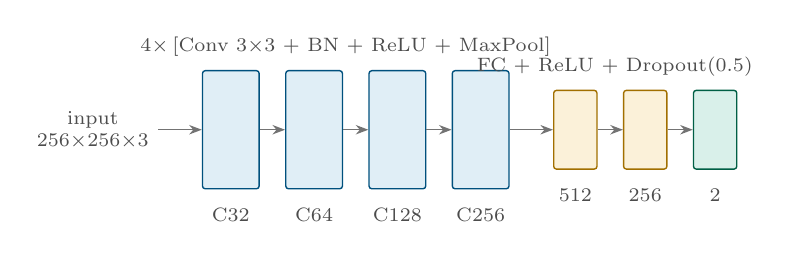
\begin{tikzpicture}[
  font=\scriptsize,node distance=0.32cm,
  conv/.style={draw=cblue!70!black,fill=cblue!12,minimum height=1.5cm,
               minimum width=0.72cm,rounded corners=1pt,line width=0.5pt},
  fc/.style={draw=corange!70!black,fill=corange!15,minimum height=1.0cm,
             minimum width=0.55cm,rounded corners=1pt,line width=0.5pt},
  lab/.style={font=\scriptsize,text=black!70,align=center},
  arr/.style={-{Stealth[length=1.6mm]},black!55,line width=0.5pt}]
  \node[lab] (in) {input\\$256{\times}256{\times}3$};
  \node[conv,right=0.55cm of in] (c1) {};
  \node[conv,right=of c1] (c2) {};
  \node[conv,right=of c2] (c3) {};
  \node[conv,right=of c3] (c4) {};
  \node[fc,right=0.55cm of c4] (f1) {};
  \node[fc,right=of f1] (f2) {};
  \node[fc,right=of f2,fill=cgreen!15,draw=cgreen!60!black] (out) {};
  \node[lab,below=0.12cm of c1] {C32};
  \node[lab,below=0.12cm of c2] {C64};
  \node[lab,below=0.12cm of c3] {C128};
  \node[lab,below=0.12cm of c4] {C256};
  \node[lab,below=0.12cm of f1] {512};
  \node[lab,below=0.12cm of f2] {256};
  \node[lab,below=0.12cm of out] {2};
  \node[lab,above=0.05cm of c2,xshift=0.4cm] {4$\times$\,[Conv 3$\times$3 + BN + ReLU + MaxPool]};
  \node[lab,above=0.05cm of f1,xshift=0.5cm] {FC + ReLU + Dropout(0.5)};
  \foreach \a/\b in {in/c1,c1/c2,c2/c3,c3/c4,c4/f1,f1/f2,f2/out}
     \draw[arr] (\a) -- (\b);
\end{tikzpicture}
\caption{\texttt{MedicalImageClassifier} backbone: four convolutional blocks
($32{\to}64{\to}128{\to}256$ filters, each Conv$3{\times}3$+BatchNorm+ReLU+MaxPool)
followed by three fully-connected layers ($512{\to}256{\to}2$) with dropout
$0.5$. Total: $34{,}076{,}162$ trainable parameters.}
\label{fig:arch}
\end{figure}

\begin{table}[H]
\centering\small
\caption{Shared experimental configuration.}
\label{tab:config}
\begin{tabular}{@{}ll@{}}
\toprule
\textbf{Component} & \textbf{Setting}\\
\midrule
Dataset & RSNA 2023 Abdominal Trauma Detection (processed PNG)\\
Labels & Binary: \texttt{any\_injury} (injury / no injury)\\
Train / test images & 3{,}200 / 800 (class-balanced)\\
Sampling & $\le 100$ patients/class, $\le 20$ images/patient\\
Backbone & Custom CNN, 4 conv + 3 FC, $34{,}076{,}162$ params\\
Input & $256\times256\times3$\\
Optimiser & Adam ($\beta_1{=}0.9,\ \beta_2{=}0.999$)\\
Loss & Cross-entropy, Eq.~\eqref{eq:ce}\\
Hardware & NVIDIA RTX 4050 (6\,GB), mixed precision (AMP)\\
\bottomrule
\end{tabular}
\end{table}

\begin{table}[H]
\centering\small
\caption{Method hyperparameters per experiment.}
\label{tab:hyper}
\begin{tabular}{@{}lcc@{}}
\toprule
\textbf{Hyperparameter} & \textbf{Exp.~1 (class-inc.)} & \textbf{Exp.~2 (window)}\\
\midrule
Learning rate            & 0.001 & 0.005\\
Batch size               & 16    & 32\\
Iterations / task        & 500   & 1000\\
EWC $\lambda$            & 5000  & 100\\
Fisher samples $N$       & 200   & 500\\
Replay buffer / task $B$ & 200   & 500\\
\bottomrule
\end{tabular}
\end{table}

% ===========================================================================
\section{Results}\label{sec:results}
% ===========================================================================
\subsection{Experiment 1: class-incremental}
Table~\ref{tab:ci} gives the summary metrics. The per-task accuracy matrices are
in Fig.~\ref{fig:ci-heat} and the trade-off in Fig.~\ref{fig:ci-tradeoff}.

\begin{table}[H]
\centering\small
\caption{Class-incremental results (2 tasks). Lowest forgetting in
\textbf{bold}. Arrows $\downarrow$/$\uparrow$ mark the preferred direction.}
\label{tab:ci}
\begin{tabular}{@{}l N N @{}}
\toprule
\textbf{Method} & {\textbf{Avg.\ accuracy (\%)} $\uparrow$} & {\textbf{Forgetting (\%)} $\downarrow$}\\
\midrule
Baseline      & 50.00 & 100.00\\
EWC           & 50.00 & 100.00\\
Replay        & 54.38 & 86.75\\
\rowcolor{cgreen!8}
EWC+Replay    & 50.75 & {\bfseries 29.50}\\
\bottomrule
\end{tabular}
\end{table}

\begin{figure}[H]
\centering
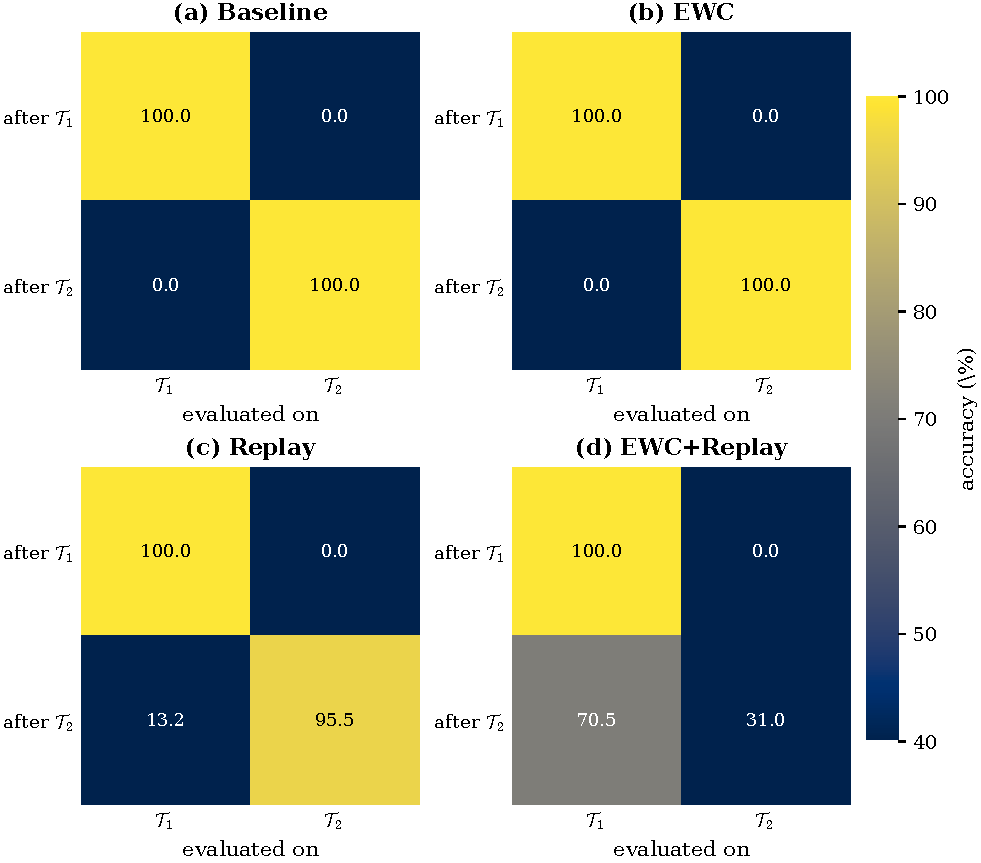
\includegraphics[width=0.86\textwidth]{ci_heatmaps.pdf}
\caption{Accuracy matrices $R_{i,j}$ for the class-incremental experiment.
Baseline and EWC wipe out Task~1 the moment they learn Task~2 ($R_{2,1}{=}0$).
Replay holds on to $13.25\%$. EWC+Replay keeps the most at $70.50\%$, but only by
giving up Task~2.}
\label{fig:ci-heat}
\end{figure}

\begin{figure}[H]
\centering
\begin{subfigure}{0.48\textwidth}\centering
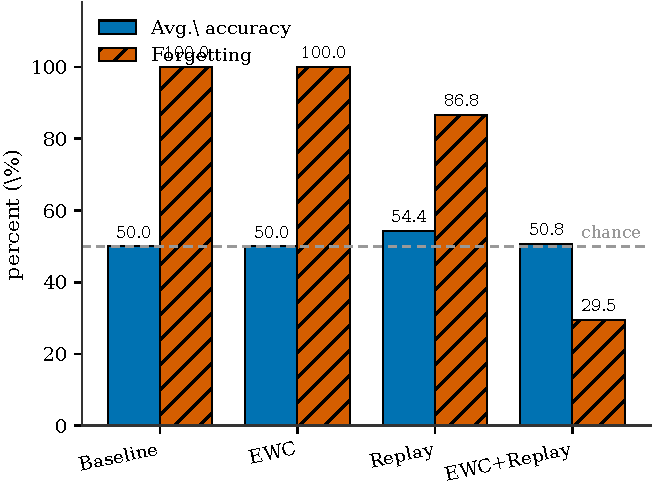
\includegraphics[width=\linewidth]{ci_summary.pdf}
\caption{Average accuracy vs.\ forgetting.}\end{subfigure}\hfill
\begin{subfigure}{0.48\textwidth}\centering
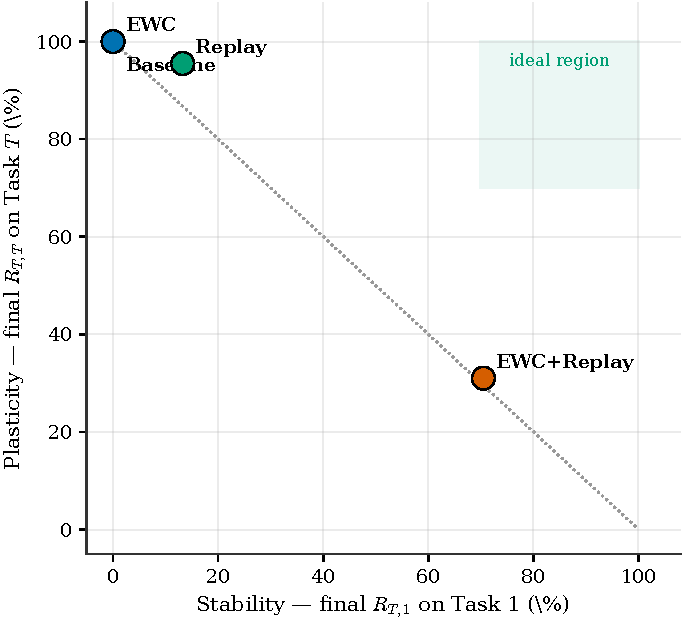
\includegraphics[width=\linewidth]{ci_stability_plasticity.pdf}
\caption{Stability--plasticity trade-off.}\end{subfigure}
\caption{Class-incremental summary. EWC+Replay is the only method that pulls
away from the full-plasticity, zero-stability corner and toward the ideal
region.}
\label{fig:ci-tradeoff}
\end{figure}

\noindent\textbf{Reading the matrices.} Reading the final row of each matrix, we
observe the stability--plasticity tension directly:
\begin{table}[H]
\centering\small
\begin{tabular}{@{}lcc@{}}
\toprule
\textbf{Method} & \textbf{Stability $R_{2,1}$} & \textbf{Plasticity $R_{2,2}$}\\
\midrule
Baseline   & 0.00\%  & 100.00\%\\
EWC        & 0.00\%  & 100.00\%\\
Replay     & 13.25\% & 95.50\%\\
EWC+Replay & 70.50\% & 31.00\%\\
\bottomrule
\end{tabular}
\end{table}
\noindent In our runs, no method manages high stability and high plasticity at
the same time.

\subsection{Experiment 2: window-based domain-incremental}
Table~\ref{tab:win} summarises this experiment and Fig.~\ref{fig:win} shows the
corresponding accuracy matrices and summary bars. The pattern is quite different
from Experiment~1, and we read it with care in Section~\ref{sec:analysis}.

\begin{table}[H]
\centering\small
\caption{Window-based results (3 tasks). Every method sits near chance
($50\%$), with Replay best on average. Low forgetting here should not be read as
success (see Section~\ref{sec:analysis}).}
\label{tab:win}
\begin{tabular}{@{}l N S[table-format=2.2] @{}}
\toprule
\textbf{Method} & {\textbf{Avg.\ accuracy (\%)} $\uparrow$} & {\textbf{Forgetting (\%)} $\downarrow$}\\
\midrule
Baseline      & 53.58 & 0.50\\
EWC           & 51.13 & -0.69\\
\rowcolor{cgreen!8}
Replay        & {\bfseries 57.71} & 1.75\\
EWC+Replay    & 53.83 & 3.00\\
\bottomrule
\end{tabular}
\end{table}

\begin{figure}[H]
\centering
\begin{subfigure}{0.62\textwidth}\centering
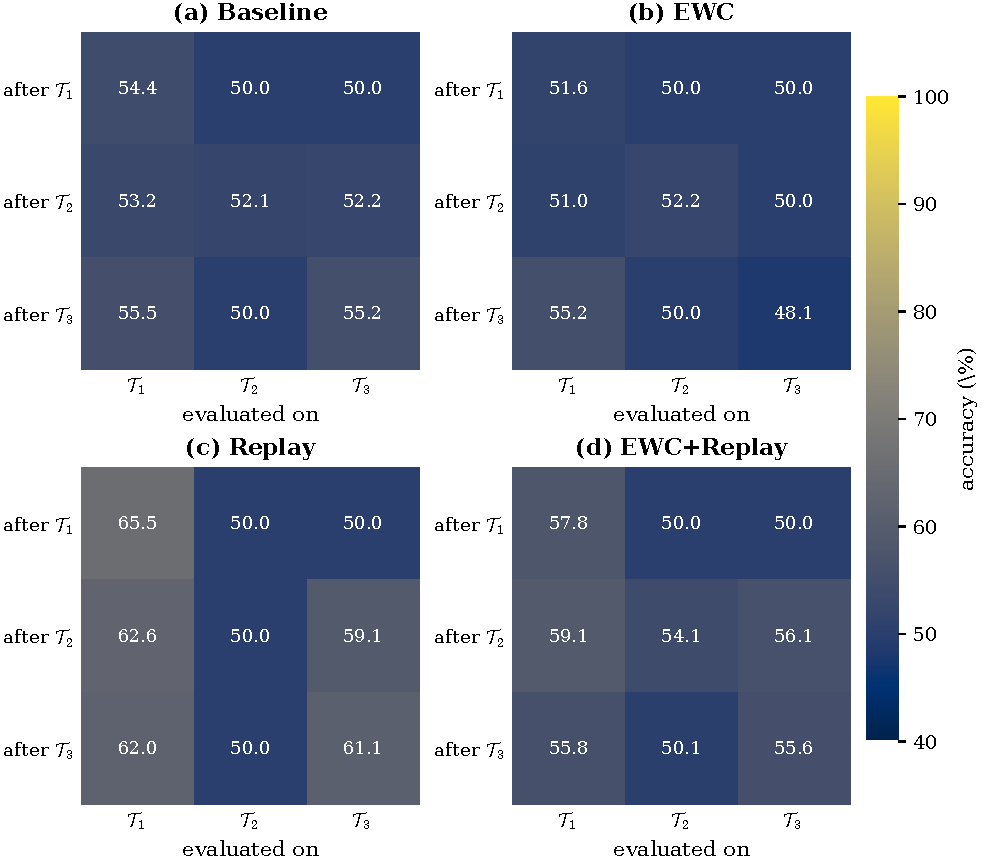
\includegraphics[width=\linewidth]{win_heatmaps.pdf}
\caption{Accuracy matrices.}\end{subfigure}\hfill
\begin{subfigure}{0.36\textwidth}\centering
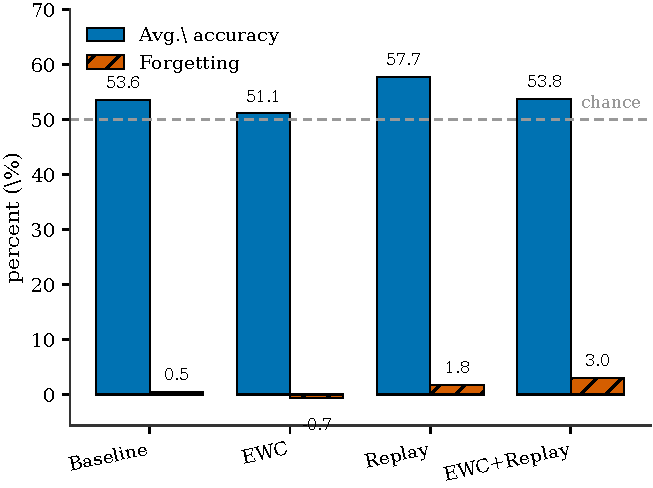
\includegraphics[width=\linewidth]{win_summary.pdf}
\caption{Summary.}\end{subfigure}
\caption{Window-based domain-incremental experiment. Most cells land at or near
$50\%$. Replay is the only method that stays above chance on the windows it has
seen.}
\label{fig:win}
\end{figure}

% ===========================================================================
\section{Analysis}\label{sec:analysis}
% ===========================================================================
\subsection{EWC in the class-incremental setting}
We observe that EWC matches the baseline at $100\%$ forgetting, and we are led to
consider two explanations that are not mutually exclusive. The first concerns
scale. At $\lambda{=}5000$ the penalty in Eq.~\eqref{eq:ewc} appears heavy enough
either to suppress new learning or, where the Fisher estimates of
Eq.~\eqref{eq:fisher} are noisy, to anchor directions that do not correspond to
genuinely important weights. Since only one label is present during Task~1, we
would expect the single-class Fisher to be a poor estimate of curvature, which
may compound the problem. The second explanation is structural. The two tasks
seem to require different output units to respond, and it is not clear how a
quadratic anchor in weight space could encode ``retain both decision regions''
while the shared softmax head is being repurposed for the new class. This is
broadly consistent with reports that weight-space regularisation struggles in the
class-incremental regime~\cite{delange2021survey}, though our single run does not
let us separate the two explanations cleanly.

\subsection{The partial protection from Replay}
Among the single methods, we observe that only Replay lowers forgetting, to
$86.75\%$, which is consistent with the intuition that Eq.~\eqref{eq:replay}
places old samples back in front of the model. The residual forgetting appears to
be tied to the imbalance in the buffer: at Task~2 the loss mixes $1{,}600$ fresh
samples with only $200$ replayed ones, so we would expect the gradient to be
dominated by the new task. We cannot rule out that a larger or better-balanced
buffer would close much of the gap, and Section~\ref{sec:mods} treats this as a
hypothesis to test rather than a settled conclusion.

\subsection{The combined method and the trade-off}
EWC+Replay reaches the lowest forgetting we measured, $29.50\%$. A plausible
reading is that replay supplies the old-class gradients while the Fisher penalty
slows their erosion, so that the two terms of Eq.~\eqref{eq:comb} act in concert.
The cost falls on plasticity, with Task~2 accuracy dropping to $31\%$. We take
this less as a recommendation than as a clear illustration that, in our setup, no
single operating point gave both high stability and high plasticity at once.

\subsection{Reading the window experiment}
In Experiment~2 we observe every method hovering around $50\%$, which suggests
that the model does not pick up the injury signal in the first place. If that is
correct, the small forgetting numbers tell us little, because a model that has
learned nothing has nothing to forget, and we are cautious about over-interpreting
them. Several factors may contribute, and we cannot apportion blame among them
from this experiment alone: a $34$M-parameter network trained on only $3{,}200$
images, a binary label that is likely weak at the level of a single slice, and a
windowing operation that restyles the input without obviously adding new
discriminative content. We therefore treat this experiment as a diagnostic, and
it leads us to consider representation quality, rather than the choice of
continual-learning algorithm, as the more pressing thing to address.

% ===========================================================================
\section{Next Modifications (implemented)}\label{sec:mods}
% ===========================================================================
Taken together the two experiments point to a fairly specific set of changes,
which we have implemented in \texttt{src/exp\_improved.py} and sketch in
Fig.~\ref{fig:pipeline}.

\begin{enumerate}[leftmargin=1.7em,topsep=2pt,itemsep=3pt]
  \item \textbf{Pretrained backbone.} Swap the custom CNN for an ImageNet
        ResNet-18~\cite{he2016resnet}. Since the window experiment shows the
        custom network appears unable to find signal in $3{,}200$ images, we
        expect a pretrained encoder to help with the representation bottleneck.
  \item \textbf{EWC $\lambda$ sweep.} Search over
        $\lambda\in\{10,50,100,500,1000\}$ rather than fixing $\lambda{=}5000$,
        which is $50\times$ the value used in the tutorial we started from and,
        we suspect, a substantial part of why EWC did not help.
  \item \textbf{Balanced replay loss.} Draw equal numbers of old and new
        examples each step and weight the memory term so the new task stops
        dominating the gradient in Eq.~\eqref{eq:replay}:
        \begin{equation}
        \mathcal{L}^{\text{bal}}_t=\tfrac{1}{2}\,
        \E_{(x,y)\sim\mathcal{D}_t}\ell(f_\theta(x),y)
        +\tfrac{1}{2}\,\E_{(x,y)\sim\mathcal{M}}\ell(f_\theta(x),y),
        \label{eq:balreplay}
        \end{equation}
        where $\E_{(x,y)\sim\mathcal{D}_t}$ denotes the expected loss over the
        current task's data $\mathcal{D}_t$, $\E_{(x,y)\sim\mathcal{M}}$ the
        expected loss over the replay buffer $\mathcal{M}$, and the equal
        $\tfrac{1}{2}$ weights give the two an equal say regardless of how many
        samples each holds ($f_\theta$ and $\ell$ as in Eq.~\eqref{eq:ce}).
  \item \textbf{Larger buffer with herding.} Raise $B$ to between $500$ and
        $1000$ per task and choose exemplars by herding, picking those nearest
        the class feature mean instead of sampling at random.
  \item \textbf{Knowledge distillation (LwF).} Keep the previous model
        $f_{\theta^{*}_{t-1}}$ as a teacher and add a temperature-$T$ soft-target
        term in the style of Hinton et al.~\cite{hinton2015distill}, following
        Learning without Forgetting~\cite{li2017lwf}. This attacks the head
        conflict in the class-incremental setting that a weight-space penalty
        cannot reach:
        \begin{equation}
        \mathcal{L}^{\text{LwF}}_t=\mathcal{L}_t(\theta)
        +\alpha\,T^2\,\mathrm{KL}\!\Big(
        \sigma\!\big(\tfrac{f_{\theta^{*}_{t-1}}(x)}{T}\big)\,\Big\|\,
        \sigma\!\big(\tfrac{f_\theta(x)}{T}\big)\Big),
        \label{eq:lwf}
        \end{equation}
        where $f_{\theta^{*}_{t-1}}$ is the frozen ``teacher'' (the model from the
        end of the previous task) and $f_\theta$ the current ``student'';
        $\sigma(\cdot)$ is the softmax; $T>1$ is a temperature that softens the
        probability distributions so the student also matches the teacher's
        relative confidences; $T^2$ rescales the term to keep its gradient
        comparable as $T$ changes; $\mathrm{KL}(\cdot\,\|\,\cdot)$ is the
        Kullback--Leibler divergence between the two softened distributions; and
        $\alpha\ge 0$ weights the distillation term against the task loss
        $\mathcal{L}_t$.
\end{enumerate}
A sixth, supporting change addresses the label signal itself. We pool
predictions to the patient and series level so that the window experiment has a
chance of rising above chance and becoming a benchmark worth measuring against.

\begin{figure}[H]
\centering
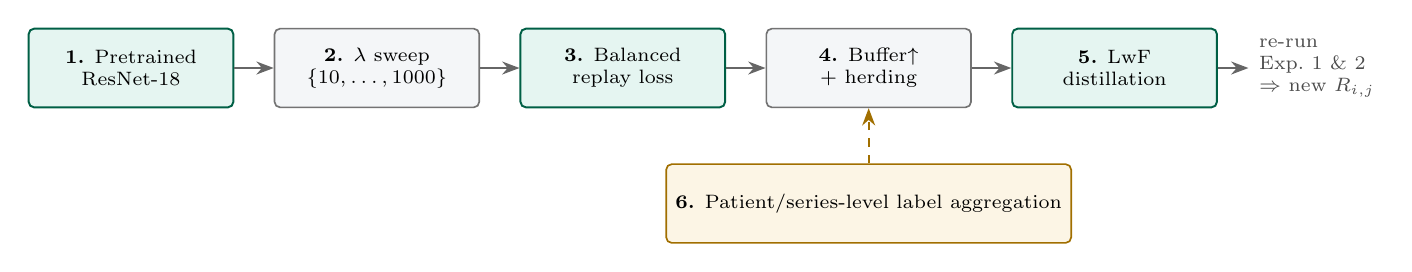
\begin{tikzpicture}[
  font=\scriptsize,node distance=0.5cm,
  stage/.style={rounded corners=2pt,draw=black!55,fill=cbg,align=center,
                minimum height=1.0cm,minimum width=2.6cm,line width=0.6pt},
  hl/.style={rounded corners=2pt,draw=cgreen!60!black,fill=cgreen!10,align=center,
             minimum height=1.0cm,minimum width=2.6cm,line width=0.7pt},
  arr/.style={-{Stealth[length=2.2mm]},line width=0.7pt,black!60}]
  \node[hl] (bb) {\textbf{1.} Pretrained\\ResNet-18};
  \node[stage,right=of bb] (sweep) {\textbf{2.} $\lambda$ sweep\\$\{10,\dots,1000\}$};
  \node[hl,right=of sweep] (bal) {\textbf{3.} Balanced\\replay loss};
  \node[stage,right=of bal] (herd) {\textbf{4.} Buffer$\uparrow$\\+ herding};
  \node[hl,right=of herd] (lwf) {\textbf{5.} LwF\\distillation};
  \foreach \a/\b in {bb/sweep,sweep/bal,bal/herd,herd/lwf}
     \draw[arr] (\a) -- (\b);
  \node[stage,below=0.7cm of herd,minimum width=4.0cm,draw=corange!70!black,
        fill=corange!10] (agg) {\textbf{6.} Patient/series-level label aggregation};
  \draw[arr,corange!70!black,dashed] (agg.north) -- (herd.south);
  \node[right=0.4cm of lwf,align=left,text=black!70]
    {\scriptsize re-run\\\scriptsize Exp.~1 \& 2\\\scriptsize $\Rightarrow$ new $R_{i,j}$};
  \draw[arr] (lwf) -- ++(1.7,0);
\end{tikzpicture}
\caption{Next-iteration pipeline. The green stages are the core algorithmic
changes and the orange stage is a supporting change to the data. All six are
implemented in \texttt{src/exp\_improved.py}.}
\label{fig:pipeline}
\end{figure}

% ===========================================================================
\section{A First Run of the Improved Pipeline}\label{sec:improved}
% ===========================================================================
We ran the improved pipeline on the same two-task class-incremental split, with a
pretrained ResNet-18 in place of the custom CNN and the EWC penalty swept across
$\lambda\in\{10,50,100,500,1000\}$. Twelve of the thirteen configurations
completed; the buffer-selection step for the largest combined run
($\lambda{=}1000$) stalled and was excluded. We report the twelve recovered runs
in Table~\ref{tab:imp} and show four representative accuracy matrices in
Fig.~\ref{fig:imp}.

The outcome is not the graded comparison we had hoped for, and we think it is
worth reporting plainly. Every configuration ends with the model perfect on one
task and at chance on the other, so the average accuracy sits at $50\%$
throughout. The methods split into two camps: fine-tuning and EWC (at every
$\lambda$) swing fully to the second task and lose the first ($R_{2}=[0,100]$),
while Replay and LwF do the opposite, holding the first task and learning almost
none of the second ($R_{2}=[100,0]$). Only the combined method at $\lambda{=}10$
and $\lambda{=}500$ lands anywhere in between, and even then it barely touches the
second task.

\begin{table}[H]
\centering\small
\caption{Improved pipeline on the two-task class-incremental split (pretrained
ResNet-18). Final accuracies are on [Task~1, Task~2]; average accuracy and
forgetting follow Eqs.~\eqref{eq:avgacc}--\eqref{eq:forget}. The
$\lambda{=}1000$ combined run is omitted (stalled).}
\label{tab:imp}
\begin{tabular}{@{}l c N N@{}}
\toprule
\textbf{Method} & \textbf{Final [T1, T2]} &
{\textbf{Avg.\ acc.\ (\%)}} & {\textbf{Forgetting (\%)}}\\
\midrule
Baseline                    & $[0,\ 100]$    & 50.00 & 100.00\\
Replay                      & $[100,\ 0]$    & 50.00 & 0.00\\
LwF                         & $[100,\ 0]$    & 50.00 & 0.00\\
EWC ($\lambda{=}10$)        & $[0,\ 100]$    & 50.00 & 100.00\\
EWC ($\lambda{=}50$)        & $[0,\ 100]$    & 50.00 & 100.00\\
EWC ($\lambda{=}100$)       & $[0,\ 100]$    & 50.00 & 100.00\\
EWC ($\lambda{=}500$)       & $[0,\ 100]$    & 50.00 & 100.00\\
EWC ($\lambda{=}1000$)      & $[0,\ 100]$    & 50.00 & 100.00\\
EWC+Replay ($\lambda{=}10$) & $[99.25,\ 0]$  & 49.62 & 0.75\\
EWC+Replay ($\lambda{=}50$) & $[0,\ 100]$    & 50.00 & 100.00\\
EWC+Replay ($\lambda{=}100$)& $[0,\ 100]$    & 50.00 & 100.00\\
EWC+Replay ($\lambda{=}500$)& $[91.25,\ 4]$  & 47.62 & 8.75\\
\bottomrule
\end{tabular}
\end{table}

\begin{figure}[H]
\centering
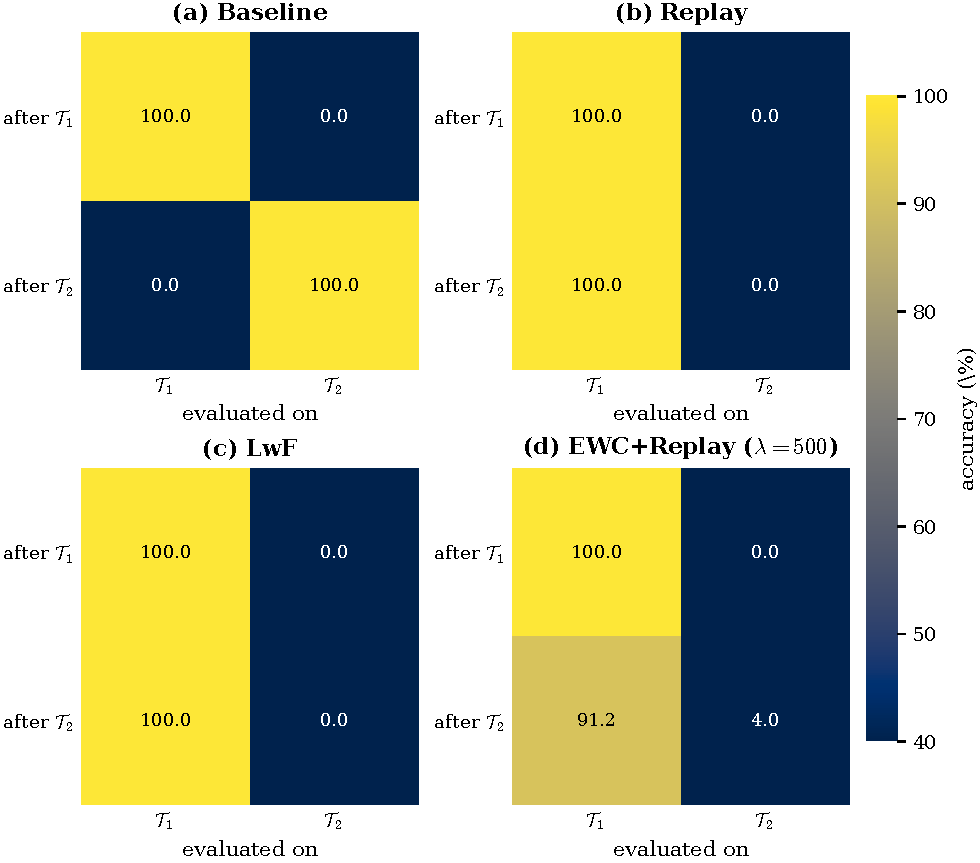
\includegraphics[width=0.82\textwidth]{imp_heatmaps.pdf}
\caption{Representative accuracy matrices from the improved pipeline. Fine-tuning
and EWC keep only the most recent task; Replay and LwF keep only the first; the
combined method at $\lambda{=}500$ retains most of Task~1 but barely learns
Task~2.}
\label{fig:imp}
\end{figure}

\noindent\textbf{How we read this.} We are inclined to attribute the collapse to
the task design rather than to the methods. With only two tasks, each containing a
single class, and a shared two-way softmax head, the balanced-replay and
distillation losses appear to lock the head onto the first task, while the
cross-entropy term on its own pulls it entirely to the second; there seems to be
no stable operating point in between. The pretrained backbone, being far more
expressive than the earlier CNN, only sharpens this effect, since it can fit
whichever single task is currently in front of it almost exactly. We also note
that patient-level aggregation cannot help here, because each task is single-class
and a majority vote over one class is uninformative. Taken together, this run
leads us to think the next useful step is to change the \emph{task design} (more
classes per task, or the multi-window domain-incremental stream of
Experiment~2) before drawing any comparison between the methods themselves. We
report it as a diagnostic rather than as evidence for or against any method.

% ===========================================================================
\section{Patient-Level Multiple-Instance Learning}\label{sec:mil}
% ===========================================================================
The diagnostics above point at the \emph{label} as the real obstacle. The
\texttt{any\_injury} flag is defined per patient, yet the slice-level models
attach it to every slice of that patient yet most slices of an injured patient
show no injury at all, so a large fraction of the positive training examples are,
in effect, mislabelled. This motivates a reformulation as multiple-instance
learning (MIL): we treat each patient as a \emph{bag} of slices with a single
bag label, and let the model decide which slices matter.

\subsection{Model}
We encode each slice with a pretrained ResNet-18 and pool the slice features into
one bag embedding with gated attention~\cite{ilse2018mil}. For a bag of $k$
slices with feature vectors $h_1,\dots,h_k\in\mathbb{R}^{D}$, the attention
weight of slice $i$ is
\begin{equation}
a_i=\frac{\exp\!\big(w^{\top}\,[\tanh(V h_i)\odot\sigma(U h_i)]\big)}
        {\sum_{j=1}^{k}\exp\!\big(w^{\top}\,[\tanh(V h_j)\odot\sigma(U h_j)]\big)},
\qquad
z=\sum_{i=1}^{k} a_i\,h_i ,
\label{eq:mil}
\end{equation}
where $h_i\in\mathbb{R}^{D}$ is the encoder feature of slice $i$ ($D{=}512$ for
ResNet-18); $V,U\in\mathbb{R}^{A\times D}$ are learned projection matrices into an
attention space of size $A$ ($A{=}128$ here); $w\in\mathbb{R}^{A}$ is a learned
scoring vector; $\tanh(\cdot)$ and $\sigma(\cdot)$ are the hyperbolic-tangent and
logistic-sigmoid functions applied elementwise; $\odot$ is the elementwise
(Hadamard) product, which forms the gating that lets the network suppress
uninformative slices; $a_i\in[0,1]$ are the resulting attention weights, summing
to one over the bag; and $z\in\mathbb{R}^{D}$ is the attention-pooled bag
embedding, passed to a linear classifier for the patient-level prediction. The
continual stream is the same three CT windows as Experiment~2, so the four
methods carry over, now applied at the bag level. We report patient-level
accuracy and the area under the ROC curve (AUC), which is threshold-free and
robust to the $73{:}27$ class imbalance.

\subsection{Results}
We ran two configurations: an initial run with $286$ training and $88$ test
patients, and a second, tuned run that used the best validation configuration
from a hyperparameter sweep (ResNet-18 encoder, encoder learning rate
$3\times10^{-5}$, $40$ slices per bag, attention size $128$) together with about
four times as much data ($1{,}106$ training, $340$ test patients). Test
patient-level AUC for both is shown in Fig.~\ref{fig:mil} and
Table~\ref{tab:mil}.

\begin{table}[H]
\centering\small
\caption{Patient-level Attention-MIL, test AUC by method, for the initial and
the tuned (larger) run. Higher is better; $50$ is chance.}
\label{tab:mil}
\begin{tabular}{@{}l S[table-format=2.1] S[table-format=2.1]@{}}
\toprule
\textbf{Method} & {\textbf{Run A AUC} (88 test)} & {\textbf{Run B AUC} (340 test)}\\
\midrule
Baseline    & 44.3 & 55.5\\
EWC         & 55.4 & 52.8\\
Replay      & 62.9 & 53.7\\
LwF         & 50.5 & 52.9\\
EWC+Replay  & 58.7 & 54.3\\
\bottomrule
\end{tabular}
\end{table}

\begin{figure}[H]
\centering
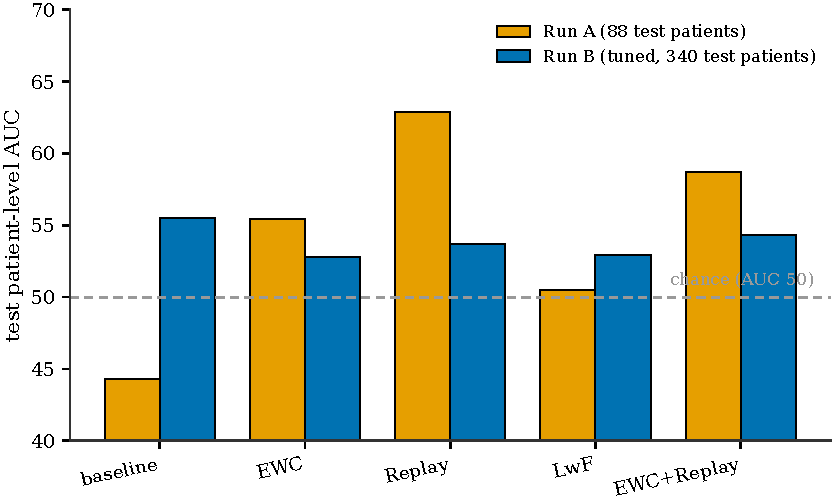
\includegraphics[width=0.66\textwidth]{mil_compare.pdf}
\caption{Test patient-level AUC for the two MIL runs. In the smaller run the
methods spread out and Replay leads at $62.9$; with four times the test patients
the same methods regress into a narrow band just above chance.}
\label{fig:mil}
\end{figure}

\subsection{Discussion: a performance ceiling}
We read these two runs together with some caution. In the smaller run the methods
separate and Replay reaches AUC $62.9$, which is encouraging. The tuned run,
however, has both more training data and a four-times larger test set, and there
the methods collapse into a narrow band ($52.8$--$55.5$) that includes the
baseline. We are inclined to read the earlier $62.9$ as partly favourable
variance on a small test set, with the larger run giving the more trustworthy
estimate. We also note that validation AUC during the tuned run peaked near $66$
yet did not carry over to the test patients, the same generalisation gap seen at
the slice level.

Taken across all our experiments, the evidence suggests a performance ceiling
near chance-to-modest (AUC of roughly $0.55$) for this particular combination of
ingredients: two-dimensional CT-window slices, a generic ResNet encoder, a coarse
patient-level \texttt{any\_injury} label, and the data and compute available to a
single 6\,GB GPU. We do not read this as a failure of the continual-learning
methods, which behave sensibly relative to one another where any signal exists;
rather, the base task itself appears not to be learnable to a clinically useful
level under these constraints. Reaching the much higher accuracies reported
elsewhere for abdominal-trauma CT would, we suspect, require volumetric (3D)
models that use inter-slice context, labels localised to the slices or organs
where injury is visible, and substantially more data and compute than were
available here. We flag these as the directions most likely to move the ceiling,
and we are careful not to claim more than our experiments support.

% ===========================================================================
\section{Conclusions}
% ===========================================================================
Within the limits of a single seeded run, our observations are consistent with a
few tentative conclusions. Under class-incremental training, plain fine-tuning
forgets almost everything, and EWC on its own does not appear to help at the
regularisation strength we used. Replay seems to be the component that buys
retention, and pairing it with EWC preserved the most old knowledge in our runs,
albeit at a clear cost to learning the new task. The window-based experiment
points in a different direction: there the limiting factor looks like
representation rather than forgetting, and we suspect the continual-learning
machinery has little to act on until the backbone and the label signal improve.
We are careful not to over-generalise from these experiments; the six changes in
Section~\ref{sec:mods} are best read as hypotheses these readings lead us to test.
A first run of the improved pipeline (Section~\ref{sec:improved}) makes one thing
clearer: swapping in a stronger backbone is not by itself enough, and the
two-task, single-class-per-task design seems to force the collapse we observe.
Reformulating the problem as patient-level multiple-instance learning
(Section~\ref{sec:mil}) addresses the label mismatch and lets the methods behave
sensibly relative to one another, but it also exposes what looks like a
performance ceiling: across our runs, test AUC settles near $0.55$, and a tuned
run with four times the data does not move it. We therefore suspect the binding
constraint is the combination of a coarse patient-level label, two-dimensional
slice input, and limited data and compute, rather than the choice of
continual-learning method. We are careful not to over-generalise from these
experiments. The most promising directions for future work, in our view, are
volumetric models that exploit inter-slice context, labels localised to where
injury is actually visible, and larger-scale training.

\paragraph{Reproducibility.} The data figures are regenerated from the recorded
results by \texttt{report/make\_figures.py} as vector PDFs, and the diagrams are
drawn natively in TikZ. The experiment code is under \texttt{src/}
(\texttt{exp\_class\_incremental.py}, \texttt{exp\_window\_3task\_v2.py},
\texttt{exp\_improved.py}, and the MIL model \texttt{exp\_mil.py} with its
validation sweep \texttt{tune\_mil.py}); raw logs, result CSVs and accuracy
matrices are in \texttt{logs/}.

% ===========================================================================
\begin{thebibliography}{99}
\bibitem{mccloskey1989} M.~McCloskey and N.~J.~Cohen.
  Catastrophic interference in connectionist networks: the sequential learning
  problem. \emph{Psychology of Learning and Motivation}, 24:109--165, 1989.
\bibitem{french1999} R.~M.~French.
  Catastrophic forgetting in connectionist networks.
  \emph{Trends in Cognitive Sciences}, 3(4):128--135, 1999.
\bibitem{kirkpatrick2017} J.~Kirkpatrick, R.~Pascanu, N.~Rabinowitz, et al.
  Overcoming catastrophic forgetting in neural networks.
  \emph{Proceedings of the National Academy of Sciences (PNAS)},
  114(13):3521--3526, 2017.
\bibitem{zenke2017si} F.~Zenke, B.~Poole, and S.~Ganguli.
  Continual learning through synaptic intelligence.
  In \emph{Proc.\ ICML}, pages 3987--3995, 2017.
\bibitem{li2017lwf} Z.~Li and D.~Hoiem.
  Learning without forgetting.
  \emph{IEEE Trans.\ Pattern Analysis and Machine Intelligence (TPAMI)},
  40(12):2935--2947, 2018.
\bibitem{rebuffi2017icarl} S.-A.~Rebuffi, A.~Kolesnikov, G.~Sperl, and
  C.~H.~Lampert. iCaRL: incremental classifier and representation learning.
  In \emph{Proc.\ IEEE CVPR}, pages 2001--2010, 2017.
\bibitem{lopezpaz2017} D.~Lopez-Paz and M.~Ranzato.
  Gradient episodic memory for continual learning.
  In \emph{Advances in Neural Information Processing Systems (NeurIPS)}, 2017.
\bibitem{chaudhry2019tiny} A.~Chaudhry, M.~Rohrbach, M.~Elhoseiny, et al.
  On tiny episodic memories in continual learning.
  \emph{arXiv:1902.10486}, 2019.
\bibitem{ilse2018mil} M.~Ilse, J.~M.~Tomczak, and M.~Welling.
  Attention-based deep multiple instance learning.
  In \emph{Proc.\ ICML}, pages 2127--2136, 2018.
\bibitem{hinton2015distill} G.~Hinton, O.~Vinyals, and J.~Dean.
  Distilling the knowledge in a neural network.
  In \emph{NeurIPS Deep Learning Workshop}, 2015.
\bibitem{he2016resnet} K.~He, X.~Zhang, S.~Ren, and J.~Sun.
  Deep residual learning for image recognition.
  In \emph{Proc.\ IEEE CVPR}, pages 770--778, 2016.
\bibitem{delange2021survey} M.~De~Lange, R.~Aljundi, M.~Masana, et al.
  A continual learning survey: defying forgetting in classification tasks.
  \emph{IEEE Trans.\ Pattern Analysis and Machine Intelligence (TPAMI)},
  44(7):3366--3385, 2022.
\bibitem{lee2020clcardiac} C.~S.~Lee and A.~Y.~Lee.
  Clinical applications of continual learning machine learning.
  \emph{The Lancet Digital Health}, 2(6):e279--e281, 2020.
\end{thebibliography}

\end{document}
